\chapter{Inheritance and Polymorphism in Python}

\section{Introduction: Real-Life Hook}

Think about a school:

\begin{itemize}
    \item All students have name, age, grade  
    \item Some students are part of sports teams  
    \item Some students are part of the music club  
\end{itemize}

Instead of writing the same attributes and methods for each type of student, \textbf{inheritance} lets us \textbf{reuse and extend a base class}.  

\textbf{Polymorphism} allows the same method name to \textbf{work differently for different objects}.

\section{Concept: Inheritance}

\begin{definition}{Inheritance}
Inheritance allows a class (child) to \textbf{inherit attributes and methods} from another class (parent), avoiding code duplication.
\end{definition}

\subsection{Example: Parent and Child Classes}

\begin{verbatim}
class Student:
    def __init__(self, name, age, grade):
        self.name = name
        self.age = age
        self.grade = grade

    def greet(self):
        print(f"Hello, I am {self.name}, grade {self.grade}")

# Child class inherits Student
class SportsStudent(Student):
    def __init__(self, name, age, grade, sport):
        super().__init__(name, age, grade)  # Call parent constructor
        self.sport = sport

    def play(self):
        print(f"{self.name} plays {self.sport}")

# Creating objects
student1 = SportsStudent("Amina", 15, "9th", "Football")
student1.greet()  # Inherited method
student1.play()   # Child method
\end{verbatim}

- \texttt{super()} calls the parent class constructor  
- Child class can add \textbf{new attributes or methods}  

\section{Concept: Polymorphism}

\begin{definition}{Polymorphism}
Polymorphism allows \textbf{different classes to use the same method name} but perform different tasks.
\end{definition}

\subsection{Example: Same Method, Different Behavior}

\begin{verbatim}
class MusicStudent(Student):
    def greet(self):
        print(f"{self.name} is in the music club, grade {self.grade}")

# Objects
student2 = MusicStudent("Rafi", 14, "8th")

# Polymorphic greet method
student1.greet()  # SportsStudent inherited greet
student2.greet()  # MusicStudent overridden greet
\end{verbatim}

- Both \texttt{student1} and \texttt{student2} have a \texttt{greet()} method  
- The method behaves according to the \textbf{object’s class}

\section{Mini-Project: Club Management System}

Create a program that stores students in different clubs and prints their info:

\begin{verbatim}
class Student:
    def __init__(self, name, grade):
        self.name = name
        self.grade = grade

    def info(self):
        print(f"{self.name}, grade {self.grade}")

class SportsStudent(Student):
    def __init__(self, name, grade, sport):
        super().__init__(name, grade)
        self.sport = sport

    def info(self):
        super().info()
        print(f"Sports: {self.sport}")

class MusicStudent(Student):
    def __init__(self, name, grade, instrument):
        super().__init__(name, grade)
        self.instrument = instrument

    def info(self):
        super().info()
        print(f"Instrument: {self.instrument}")

students = [
    SportsStudent("Amina", "9th", "Football"),
    MusicStudent("Rafi", "8th", "Guitar")
]

for student in students:
    student.info()
\end{verbatim}

Output:

\begin{verbatim}
Amina, grade 9th
Sports: Football
Rafi, grade 8th
Instrument: Guitar
\end{verbatim}

\section{Step-by-Step Diagram: Inheritance and Polymorphism}

\begin{center}
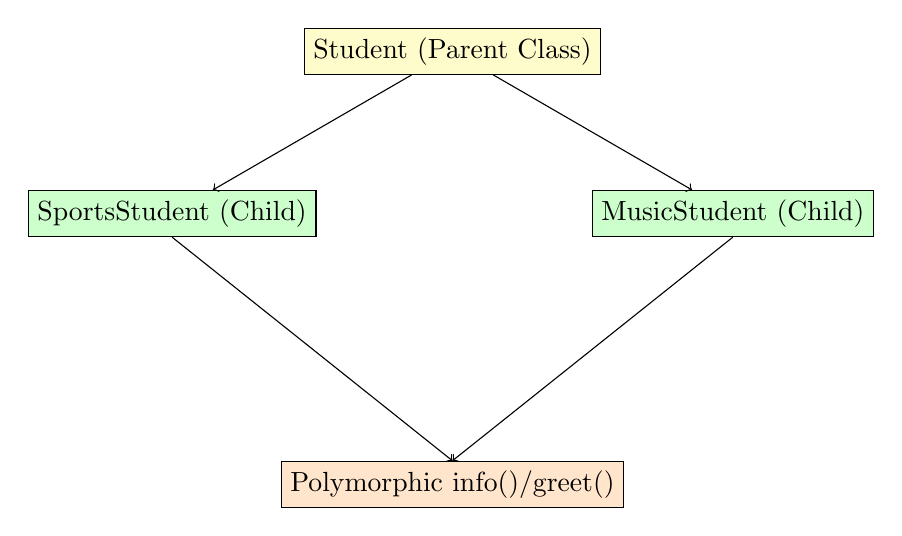
\begin{tikzpicture}[node distance=1.5cm]
\node (student) [draw, rectangle, fill=yellow!20] {Student (Parent Class)};
\node (sports) [draw, rectangle, fill=green!20, below left of=student, xshift=-2.5cm, yshift=-1cm] {SportsStudent (Child)};
\node (music) [draw, rectangle, fill=green!20, below right of=student, xshift=2.5cm, yshift=-1cm] {MusicStudent (Child)};
\node (method) [draw, rectangle, fill=orange!20, below of=student, yshift=-4cm] {Polymorphic info()/greet()};
\draw[->] (student) -- (sports);
\draw[->] (student) -- (music);
\draw[->] (sports.south) -- (method.north);
\draw[->] (music.south) -- (method.north);
\end{tikzpicture}
\end{center}

\section{Key Concepts}

\begin{itemize}
    \item \textbf{Inheritance}: child class reuses parent attributes and methods  
    \item \textbf{Polymorphism}: same method can behave differently in different classes  
    \item \texttt{super()} calls the parent constructor or methods  
    \item Helps \textbf{avoid code duplication} and \textbf{increase modularity}  
\end{itemize}

\section{End-of-Chapter Exercises}

\begin{exercise}{Very Short Questions}
\begin{enumerate}
    \item What is inheritance in Python?  
    \item What is polymorphism?  
    \item How do you call the parent class constructor in a child class?  
\end{enumerate}
\end{exercise}

\begin{exercise}{Short Answer Questions}
\begin{enumerate}
    \item Create a base class \texttt{Vehicle} with attribute \texttt{brand} and method \texttt{info()}.  
    \item Create a child class \texttt{Car} that adds \texttt{model} attribute and overrides \texttt{info()}.  
    \item Explain the difference between overriding and overloading.  
\end{enumerate}
\end{exercise}

\begin{exercise}{Activity-Based Questions}
\begin{enumerate}
    \item Create a \texttt{Teacher} base class with name and subject. Create \texttt{MathTeacher} and \texttt{MusicTeacher} child classes, each with a method \texttt{info()} that prints different details.  
    \item Extend the Student Club Management program to add a \texttt{ScienceClubStudent} class with attribute \texttt{project}. Use polymorphism to display info for all students.  
    \item Create a base class \texttt{Appliance} with \texttt{brand} and \texttt{power}. Create \texttt{Fan} and \texttt{Light} child classes, each with overridden \texttt{info()} method.  
\end{enumerate}
\end{exercise}

\section{Teacher Notes}

\marginnote{
\textbf{Learning Objectives:}  
\begin{itemize}
    \item Students understand inheritance and reuse of code  
    \item Students can create child classes and override methods  
    \item Students can implement polymorphism in Python  
\end{itemize}

\textbf{Teaching Tips:}  
\begin{itemize}
    \item Use real-life examples like students in clubs, teachers, vehicles  
    \item Show how child classes inherit and extend parent class functionality  
    \item Demonstrate polymorphic methods with multiple object types  
\end{itemize}

\textbf{Assessment:}  
\begin{itemize}
    \item Check correct implementation of child classes and polymorphic methods  
    \item Observe understanding of code reuse and modularity  
\end{itemize}
}